\documentclass{article}
\usepackage{graphicx} % Required for inserting images
\usepackage{listings}
\usepackage{amsmath}
\usepackage{bm}
\usepackage{todonotes}
\usepackage{tikz}
\usepackage{hyperref}
\usepackage[english,capitalize,noabbrev]{cleveref}
\usepackage[\languagename,capitalize,noabbrev]{cleveref}
\usetikzlibrary{positioning, arrows.meta}


\begin{document}

%%%%%%%%%%%%%%%%%%%%%%%%%%%%%%%%%%%%%%%%%%%%%%%%%
%
%       Bitte hier die eigenen Daten eingeben
%       (für Generierung der Titelseite etc.)
%
%%%%%%%%%%%%%%%%%%%%%%%%%%%%%%%%%%%%%%%%%%%%%%%%%

\newcommand{\autor}{Nils Reck}% Vorname Name
\newcommand{\mnr}{2898155} % Matrikelnummer, bspw.: 12345

%%%%%%%%%%%%%%%%%%%%%%%%%%%%%%%%%% 
%
% Hier können weitere Autoren (und eine Gruppe) definiert werden. Diese können durch Anpassung der Titelseite.tex und der Erklaerung.tex berücksichtigt werden:
%
%\newcommand{\autorII}{Erika Musterfrau}% Vorname Name
%\newcommand{\mnrII}{54321} % Matrikelnummer, bspw.: 54321
%
%\newcommand{\gruppenr}{00}
%
%%%%%%%%%%%%%%%%%%%%%%%%%%%%%%%%%%

\newcommand{\betreuerI}{Dr. Carel van Niekerk} % Name betreuender Prof

\newcommand{\betreuerII}{Dr. Hsien-Chin Lin} % Name 2. Betreuer

\newcommand{\modulname}{Implementing Transformers} % Hier den Modulnamen eingeben

\newcommand{\projektname}{Project Report} % Hier den Belegtitel eingeben

\newcommand{\datum}{29.\,01.\,2025}

% Fakultät und Studiengang:

\newcommand{\fak}{Dialog Systems and Machine Learning} % Eingabe der Fakultät
\newcommand{\studiengang}{Computer Science, MSc} % Eingabe des Studiengangs


\begin{titlepage}
\begin{center}

\includegraphics[width=.9\textwidth]{figures/HHU_Logo_WortBildMarke} \par
\vspace{2.5cm}
\textsc{\LARGE Faculty \fak} \par
\vspace{1.5cm}
\textsc{\Large \modulname} \par
\vspace{3cm}
{ \huge \bfseries \projektname} \par
\vspace{1.5cm}
%%%%%%%%%%%%%%%%%%%%%%%%%%%%%%%%%%
\renewcommand{\arraystretch}{1.5}
%Entsprechend der Anzahl der Autoren anpassen bzw. Kommentarzeichen (%) entfernen
\begin{table}[h]
\large
    \centering
    \begin{tabular}{lll}
        &
        %\underline{Gruppe \gruppenr} % Gruppennummer
        & \\
        \emph{Author} % ggf. "Autoren"
        & \autor & \mnr \\
        %& \autorII & \mnrII \\
        %...
        \vspace{-0.5cm} \\
        \emph{Supervisors} & \betreuerI & \betreuerII 
    \end{tabular}
\end{table}
\renewcommand{\arraystretch}{1} \par
%%%%%%%%%%%%%%%%%%%%%%%%%%%%%%%%%%
\vfill
{\large \datum}
\end{center}
\end{titlepage}


\section{Introduction}

The Transformer model~\cite{vaswani2017attention} established the foundation for more performant and context-aware sequence transduction by removing the recurrent or convolutional means of previous state-of-the-art models.
This is mainly due to the Transformer's ability to process multiple sequences at once.
Up until today, the Transformer model remains the architecture of choice for top-performing large language models, like GPT-4o. \\
This report showcases my attempt to implement a custom Transformer model for a German-English translation task and aligns with the practicals conducted during the course.
In particular, it focuses on providing the reader with detailed knowledge about its components and their interplay, as well as my personal insights and struggles during development and training.
Thus, the report commences with a methodology section, explaining the modular components of a Transformer and the overall architecture.

\section{Methodology} The Transformer mainly consists of two principal components, the encoder and decoder.
While both process and transform input data, the encoder focuses on generating a context-rich representation of the input sequence, whereas the decoder uses this representation to generate the target sequence step by step.
However, before the model can process the input data, it has to be encoded in a numerical representation that the model can interpret.
For this, a shared tokenizer is trained over the source and target sequences, which maps a token (a word or subword) of a sequence to a number and vice versa. 

\todo[inline]{add info about alignment of sequences (maybe add to training section)}

\subsection{Embedding Layers} 
The embedding layer creates a \texttt{$d_{model}$}-dimensional vector representation for each encoded token of the input and target sequence. 
Unlike recurrent architectures, which process sequences step by step, the Transformer processes entire sequences in parallel. 
To compensate for the lack of sequence order awareness, the positional encoding layer enriches the representations with positional information. \\
Cosistent with the original Transfromer architecture, we apply parameter sharing by using the same set of weights for both embedding layers and the pre-softmax linear transformation. This technique has shown to improve efficiency and model performance~\cite{press2017usingoutputembeddingimprove}.
Sharing parameters between the encoder and decoder embedding layers offers several advantages.
First, it can significantly reduce the model size while maintaining model performance.
Second, parmeter sharing reduces the degrees of freedom of the model, thus implicitly applying regularization by forcing different parts of the model to use the same parameters, preventing the model from overfitting.
Additionally, the efficiency of the model improves because shared parameters allow for faster updates and fewer memory operations.
Finally, by tying the input and output embeddings together, the model can enhance cross-lingual transfer learning, as aligned word representations across languages make it easier to generalize.

\subsection{Encoder Stack} 
The encoder is composed of six identical layers, each designed to transform the input sequence into a context-rich representation.
Each layer consists of two sub-layers: a multi-head self-attention mechanism and a position-wise feed-forward network.
To stabilize training and improve gradient flow, a residual connection~\cite{he2015deepresiduallearningimage} and layer normalization~\cite{ba2016layernormalization} are applied after each sub-layer.
Residual connections, defined by \(x + f(x)\), help keep the original signal in the data intact while still being able to add important properties in the form of features (output from multi-head attention or feed-forward networks). Additionally, during backpropagation, we alleviate the problem of vanishing gradients because we add back the original signal and the signal is kept alive. Even if a block does not learn anything (\(g(\mathbf{x}) = 0\), where all weights and biases are pushed to zero), the original signal is kept intact. Lastly, using the residual connection, the underlying attention or feed-forward layer only needs to learn the function \(g(\mathbf{x})=f(\mathbf{x})-\mathbf{x}\) (called residual mapping). It has a less complex shape than learning \(f(\mathbf{x})\) from scratch. If the desired function is close to the identity function (\(f(\mathbf{x}) \approx \mathbf{x}\)), \(g(\mathbf{x}) = f(\mathbf{x}) - \mathbf{x}\) becomes small and easier to learn. This naturally evokes the question of why a network would want to learn a function that is (close to) the identity function. The answer is that residual blocks act as refinement units, slightly refining existing features instead of learning full (high variance) functions from scratch. It also mitigates the risk of overfitting: If \(f(\mathbf{x})\) is far from \(\mathbf{x}\), the layer needs to learn complex transformations. By focussing on small residuals \(g(\mathbf{x}) = f(\mathbf{x}) - \mathbf{x}\), the network increases the chance of generalizing better to unseen data. However, even when \(f(\mathbf{x})\) is far from \(\mathbf{x}\), it still provides a fallback for easier gradient flow.
In the backward pass, if you have multiple rank-deficient matrices, your rank becomes even lower
because the composition of rank-deficient matrices leads to a further reduction in the rank, potentially causing the gradients to vanish or lose critical information needed for effective weight updates.

This is the corresponding paper: \cite{he2015deepresiduallearningimage}.
\subsection{Decoder Stack} 
The decoder also consists of six identical layers.
In addition to the two sub-layers of the encoder, it has a second multi-head attention mechanism over the outputs of the encoder.
According to the encoder, residual connections and layer normalization are employed after each sub-layer.
In contrast to the multi-head self-attention layer in the encoder, the inputs to the attention mechanism in the decoder are masked such that the decoder cannot attend to future tokens.
This prevents the decoder from cheating by attending to tokens it has not yet seen.
Finally, the output of the decoder undergoes a linear transformation. After that, softmax is applied to convert the output into probabilities to predict the next token.


% why position? Understand embeddings of the input. Add how the heads are
% concatenated in attention
\subsection{Attention} 
\todo[inline]{Explain how multiple atttention heads help}
It expands the model’s ability to focus on different positions.
Yes, in the example above, z1 contains a little bit of every other encoding, but it could be dominated by the actual word itself.
If we’re translating a sentence like “The animal didn’t cross the street because it was too tired”, it would be useful to know which word “it” refers to.

\subsection{Position-wise Feed-Forward Layer}
% layer normalization where? Write down the equation for the layer
% normalization layer and provide an explanation of the function of this layer
% in a transformer model. My question: Why is it important to use two
% independent layer normalization layers following multi-head self-attention
% layer and the position-wise feed-forward layer? Explain the benefits of
% parameter sharing in the transformer model.

\begin{center}
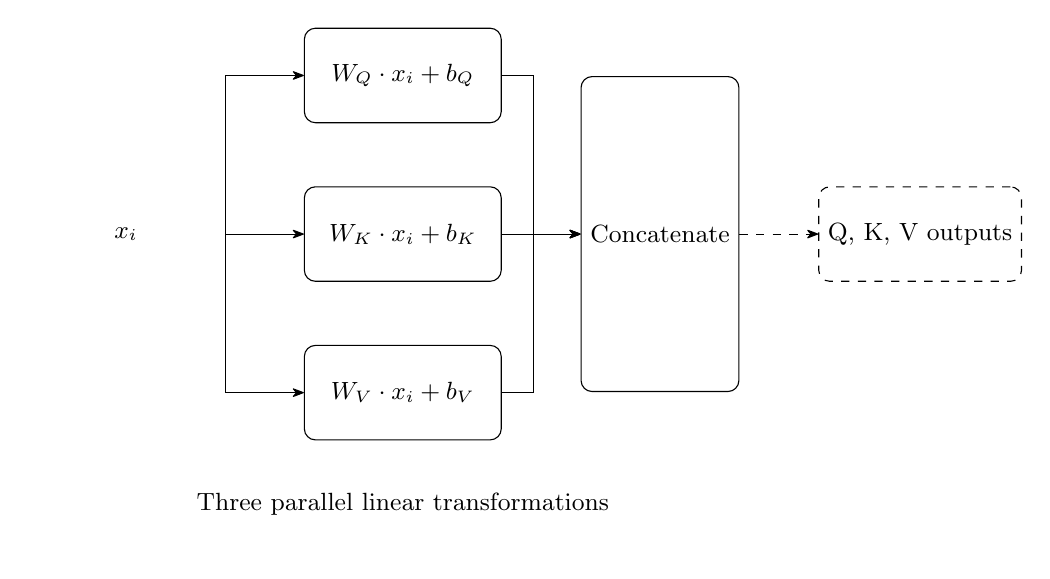
\begin{tikzpicture}[
		>={Stealth[round]}, % Arrow style
		node distance=2.5cm, % Distance between nodes
		every node/.style={draw, rounded corners, minimum width=2.5cm, minimum height=1.2cm, font=\small}
	]
			
	% Input node
	\node[draw=none] (input) {$x_i$};
			
	% Linear layer nodes
	\node[right=1cm of input] (K) {$W_K \cdot x_i + b_K$};
	\node[above=0.8cm of K] (Q) {$W_Q \cdot x_i + b_Q$};
	\node[below=0.8cm of K] (V) {$W_V \cdot x_i + b_V$};
			
	% Connect input to each linear layer
	\draw[->] (input.east) |- (Q.west);
	\draw[->] (input.east) |- (K.west);
	\draw[->] (input.east) |- (V.west);
			
	% Label nodes
	\node[below=0.2cm of V, draw=none] (labels) {Three parallel linear transformations};
			
	% Concatenate box with vertical text
	\node[draw, right=1cm of K, minimum width=1.2cm, minimum height=4cm, align=center] (concatBox) {Concatenate};
			
	% Connect linear layers to the concatenate box
	\draw[->] (Q.east) -- ++(0.4,0) |- (concatBox.west);
	\draw[->] (K.east) -- ++(0.4,0) |- (concatBox.west);
	\draw[->] (V.east) -- ++(0.4,0) |- (concatBox.west);
			
	% Dashed QKV outputs box centered vertically with Concatenate box
	\node[draw, dashed, right=1cm of concatBox, minimum width=2.5cm, minimum height=1.2cm, font=\small] (QKVBox) {Q, K, V outputs};
			
	% Arrow to QKV outputs
	\draw[->, dashed] (concatBox.east) -- (QKVBox.west);
			
\end{tikzpicture}
\end{center}

\section{Optimization Techniques}
\subsection{Learning Rate Scheduler}
\subsection{Optimizer}
% Study the AdamW optimiser used. Write down the update equations and explain
% the reasoning behind the bias correction and decoupled weight decay.

\section{Training}
% What went wrong during multiple iterations of training?

\section{Results}\label{sec:results}

This section provides the results of the CPU vs. GPU comparison, as well as the performance of the Transformer model on the translation task.

\subsection{GPU versus CPU Training}

\cref{tab:comparison} illustrates the results of the performance comparison between CPU and GPU training.
The GPU significantly accelerates the overall training process by a factor of 8.07.
Accordingly, the GPU processes a single epoch, as well as a forward pass, faster by approximately the same margin.
The GPU achieves the most significant speed-up (20x) during the backward pass.
This highlights the GPU's superior efficiency in handling computationally expensive tasks, such as gradient computation, which heavily rely on parallelized matrix calculations.
Surprisingly, the GPU uses 38 times less memory per epoch compared to the CPU, which can mainly be attributed to the small batch size of 32 for both setups.\\
Due to approaching deadlines and long queues on the high performance cluster (HPC), I postpone further optimizations of the GPU codebase.
For instance, offloading BLEU score calculations to the CPU, combined with mixed-precision training and other optimizations, can approximately halve overall training time--a speedup that has been observed in practical 11.\\
\begin{table}[ht]
    \centering
    \begin{tabular}{lccc}
        \toprule
        \textbf{Metric} & \textbf{CPU} & \textbf{GPU} & \textbf{CPU to GPU Ratio} \\
        \midrule
        Training time (hours)       & 3.0017 & 0.3717 & 8.07 \\
        Avg. Epoch times (seconds)       & 2161.24 & 267.63 & 8.07 \\
        Avg. Forward pass times (seconds)& 0.0770 & 0.0088 & 8.75 \\
        Avg. Backward pass time (seconds)& 0.2020 & 0.0101 & 20 \\
        Avg. Single step time (seconds)  & 0.2790 & 0.0189 & 14.76  \\
        Allocated memory per epoch (MB)       & 32998.0  & 865.91 & 38.1 \\
        \bottomrule
    \end{tabular}
    \caption{Performance comparison of CPU vs. GPU}
    \label{tab:comparison}
\end{table}
While the performance benefits speak for themselves, GPU training entails some disadvantages.
Working on the HPC, I experienced long queues before the jobs could start, as well as complexity in setting up the code and accompanying libraries to run on the GPU nodes.
This results in longer feedback cycles because each attempt requires submitting a new job and waiting.
If errors occur, they only got discovered after the job queue processed the experiment, further extending debugging time.
Additionally, estimating the memory resources for optimizing throughput was time-consuming and often required trial and error, especially without easy access to a GPU for testing.

\clearpage
\subsection{Machine Translation}
\cref{fig:bleu} shows that on the WMT German-to-English translation task, the Transformer model reaches a BLEU score of around 0.34 with a length ratio of 0.99 on the validation set, which implies solid, coherent translations.
Training took approximately 11.5 hours.


\begin{figure}[ht]
    \begin{center}
        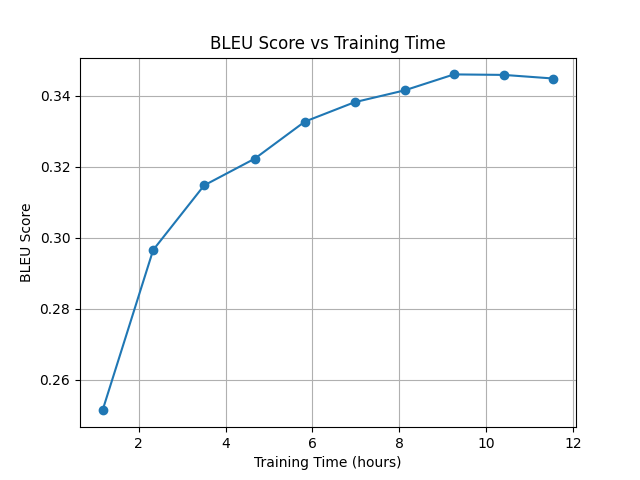
\includegraphics[width=\textwidth]{figures/bleu_score_val_20250129_142747.png}
    \end{center}
    \caption{The BLEU score is calculated on the validation set after each epoch. It approaches a value of around 0.34.}
    \label{fig:bleu}
\end{figure}
Word count: 2282


\begin{enumerate}
	\item Make sure you understand the embeddings of the input. Explain why we need the position of input characters in the embedding.
	\item Make sure you understand the role of the two different masks in the attention mechanism. Explain the role of each mask in your own words.
	\item The model starts with a Query (Q) for the current position. For example, if the model predicts the next token for the word "cat", the Query is derived from the representation of "cat".
\end{enumerate}

\section{Questions}
\subsection{Practical 4}
\begin{enumerate}
	\item Wich dimension do the word embeddings need to have?
	\item Why do values have a different dimension \(d_v\), compared to queries and keys \(d_k \), wrt the linear projection in mha?
    \item How does the model differentiate between embedding and positional encoding?
\end{enumerate}
\subsection{Practical 5}
\begin{enumerate}
	\item Why is it called encoder/decoder?
\end{enumerate}
\begin{enumerate}
	\item Do we put the tokenizer in the \lstinline{TranslationDataset} class?
	\item What is the word embedding dimension?
\end{enumerate}


\clearpage


\todo[inline]{Where do we apply dropout?}
\todo[inline]{What are learnable parameters in a transformer model?}
\todo[inline]{Inclued questions from tests}

\clearpage



\clearpage
\bibliography{references}
%% Depending on Language, use German alphadin or original alpha
\iflanguage{ngerman}{
  \bibliographystyle{alphadin}
}{
  \bibliographystyle{alpha}
}

\end{document}
